% This is "sig-alternate.tex" V1.9 April 2009
% This file should be compiled with V2.4 of "sig-alternate.cls" April 2009
%
% This example file demonstrates the use of the 'sig-alternate.cls'
% V2.4 LaTeX2e document class file. It is for those submitting
% articles to ACM Conference Proceedings WHO DO NOT WISH TO
% STRICTLY ADHERE TO THE SIGS (PUBS-BOARD-ENDORSED) STYLE.
% The 'sig-alternate.cls' file will produce a similar-looking,
% albeit, 'tighter' paper resulting in, invariably, fewer pages.
%
% ----------------------------------------------------------------------------------------------------------------
% This .tex file (and associated .cls V2.4) produces:
%       1) The Permission Statement
%       2) The Conference (location) Info information
%       3) The Copyright Line with ACM data
%       4) NO page numbers
%
% as against the acm_proc_article-sp.cls file which
% DOES NOT produce 1) thru' 3) above.
%
% Using 'sig-alternate.cls' you have control, however, from within
% the source .tex file, over both the CopyrightYear
% (defaulted to 200X) and the ACM Copyright Data
% (defaulted to X-XXXXX-XX-X/XX/XX).
% e.g.
% \CopyrightYear{2007} will cause 2007 to appear in the copyright line.
% \crdata{0-12345-67-8/90/12} will cause 0-12345-67-8/90/12 to appear in the copyright line.
%
% ---------------------------------------------------------------------------------------------------------------
% This .tex source is an example which *does* use
% the .bib file (from which the .bbl file % is produced).
% REMEMBER HOWEVER: After having produced the .bbl file,
% and prior to final submission, you *NEED* to 'insert'
% your .bbl file into your source .tex file so as to provide
% ONE 'self-contained' source file.
%
% ================= IF YOU HAVE QUESTIONS =======================
% Questions regarding the SIGS styles, SIGS policies and
% procedures, Conferences etc. should be sent to
% Adrienne Griscti (griscti@acm.org)
%
% Technical questions _only_ to
% Gerald Murray (murray@hq.acm.org)
% ===============================================================
%
% For tracking purposes - this is V1.9 - April 2009

\documentclass{Group6_Phase2}

\begin{document}
%
% --- Author Metadata here ---
%\conferenceinfo{WOODSTOCK}{'97 El Paso, Texas USA}
%\CopyrightYear{2007} % Allows default copyright year (20XX) to be over-ridden - IF NEED BE.
%\crdata{0-12345-67-8/90/01}  % Allows default copyright data (0-89791-88-6/97/05) to be over-ridden - IF NEED BE.
% --- End of Author Metadata ---

\title{Group 6 - Phase 2}
%\subtitle{[Extended Abstract]}
%
% You need the command \numberofauthors to handle the 'placement
% and alignment' of the authors beneath the title.
%
% For aesthetic reasons, we recommend 'three authors at a time'
% i.e. three 'name/affiliation blocks' be placed beneath the title.
%
% NOTE: You are NOT restricted in how many 'rows' of
% "name/affiliations" may appear. We just ask that you restrict
% the number of 'columns' to three.
%
% Because of the available 'opening page real-estate'
% we ask you to refrain from putting more than six authors
% (two rows with three columns) beneath the article title.
% More than six makes the first-page appear very cluttered indeed.
%
% Use the \alignauthor commands to handle the names
% and affiliations for an 'aesthetic maximum' of six authors.
% Add names, affiliations, addresses for
% the seventh etc. author(s) as the argument for the
% \additionalauthors command.
% These 'additional authors' will be output/set for you
% without further effort on your part as the last section in
% the body of your article BEFORE References or any Appendices.

\numberofauthors{2} %  in this sample file, there are a *total*
% of EIGHT authors. SIX appear on the 'first-page' (for formatting
% reasons) and the remaining two appear in the \additionalauthors section.
%
\author{
% You can go ahead and credit any number of authors here,
% e.g. one 'row of three' or two rows (consisting of one row of three
% and a second row of one, two or three).
%
% The command \alignauthor (no curly braces needed) should
% precede each author name, affiliation/snail-mail address and
% e-mail address. Additionally, tag each line of
% affiliation/address with \affaddr, and tag the
% e-mail address with \email.
%
%	1st. author
	\alignauthor
		Kevin Dombrosky\\
		       \affaddr{Rochester Institute of Technology Student}\\
		       \affaddr{610 Park Point Dr}\\
		       \affaddr{Rochester, New York 14623}\\
		       \email{kfd6490@rit.edu}
%	2nd. author
	\alignauthor
		Brittany Purcell\\
		       \affaddr{Rochester Institute of Technology Student}\\
		       \affaddr{107 Weldon Street}\\
		       \affaddr{Rochester, New York 14611}\\
		       \email{blp6903@rit.edu}
}

\maketitle
\begin{abstract}
This paper discusses the group project for Group 6 in the Intro to Big Data class at Rochester Institute of Technology, CSCI-620. This paper will discuss the progress, ideals, and implementation on creating a database with visual representation.
\end{abstract}

\keywords{Phase 1, Group 6, Plants}

\section{Introduction}
The group project for CSCI-620, Intro to Big Data at Rochester Institute of Technology was a semester long project where members of the group had to take a dataset, and create a way to organize and understand the dataset. The project was meant to expand the members knowledge and understanding of handling large datasets, as well as create a way for others to analyze the data.

Of the two requirements for the project, which include a database management system (DBMS), and having some form of database analytic. The members used the the Plants dataset from the UCI Machine Learning Repository which contained information on the growth location and scientific names of plants in North America. The data was then put into a relational database, MySQL. 

For the analytic the team decided on a visual representation using a webpage that displayed a map of the United States and Canada. The user can then either search for a plant name, or select a region on the map, and the results of the dataset would become available. There will be more specifics on the visualization later in the paper.  
\\\\\\\\\\\\

\section{Body}

\subsection{Database}
 As a reminder, the dataset being used is the Plants dataset from the UCI Machine Learning Repository (http://archive.ics.uci.edu/ml \\* /datasets/Plants), and was set up in a MySQL database. In order to add all of the data into a MySQL, a Java script was created. The script ran through the dataset and added the elements into MySQL. 
 
 The information found in the database consists of a plant and its location in the United States/Canada. Below is the Entity-relationship(ER) diagram which was developed by Group 6. This diagram is the basis for how the information from the dataset was stored in the database.

\begin{figure}[htb]
	\centering
	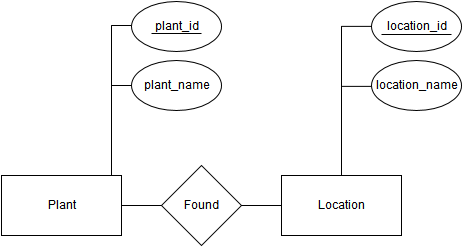
\includegraphics[scale=0.5]{FinalProject_ERdiagram.png}
	\caption{The ER diagram which represents the organization of the data in the database.}
\end{figure}

Later, when the visual needs to access the information in the dataset, this allows for proper organization so the appropriate calls can be made. There are three tables within the database. The first holds the information on the plants. The consists of the plant ID, as well as the name of the plant associated with that ID. The locations table is very similar. The location table has the location ID and the associated location. Lastly, there is a table which compares the locations and plants. This table is maps the plant-id to a location-id. This is how the location and plant information can be accessed using the appropriate calls, and will be simple to display in the visual.

There are a few specific sets of data which were excluded from the dataset. These were Greenland/Denmark, St. Pierre and Miquelon, and Prince Edward Island. The reason the members excluded these locations is because the map only looked at The United States and Canada. These regions were outside the scope of the map, and therefore were outside the scope of the project. 


\subsection{Application}
The group decided that for the analytic portion of the project they would work with a map visualization on a webpage. The map is functional only for the United States and Canada, and each region is selectable. Selecting a region would bring up the list of plants that can be found in that area. 

The visualization also has the ability to search by plant name. The search does a sub search, that will find all plant names containing what is typed in. When you search either using the full plant name, or a sub plant name, the locations where the plant is available will show up green. When searching or selecting a plant name, any locations where that plant is will show in the map. 

\begin{figure}[htb]
	\centering
	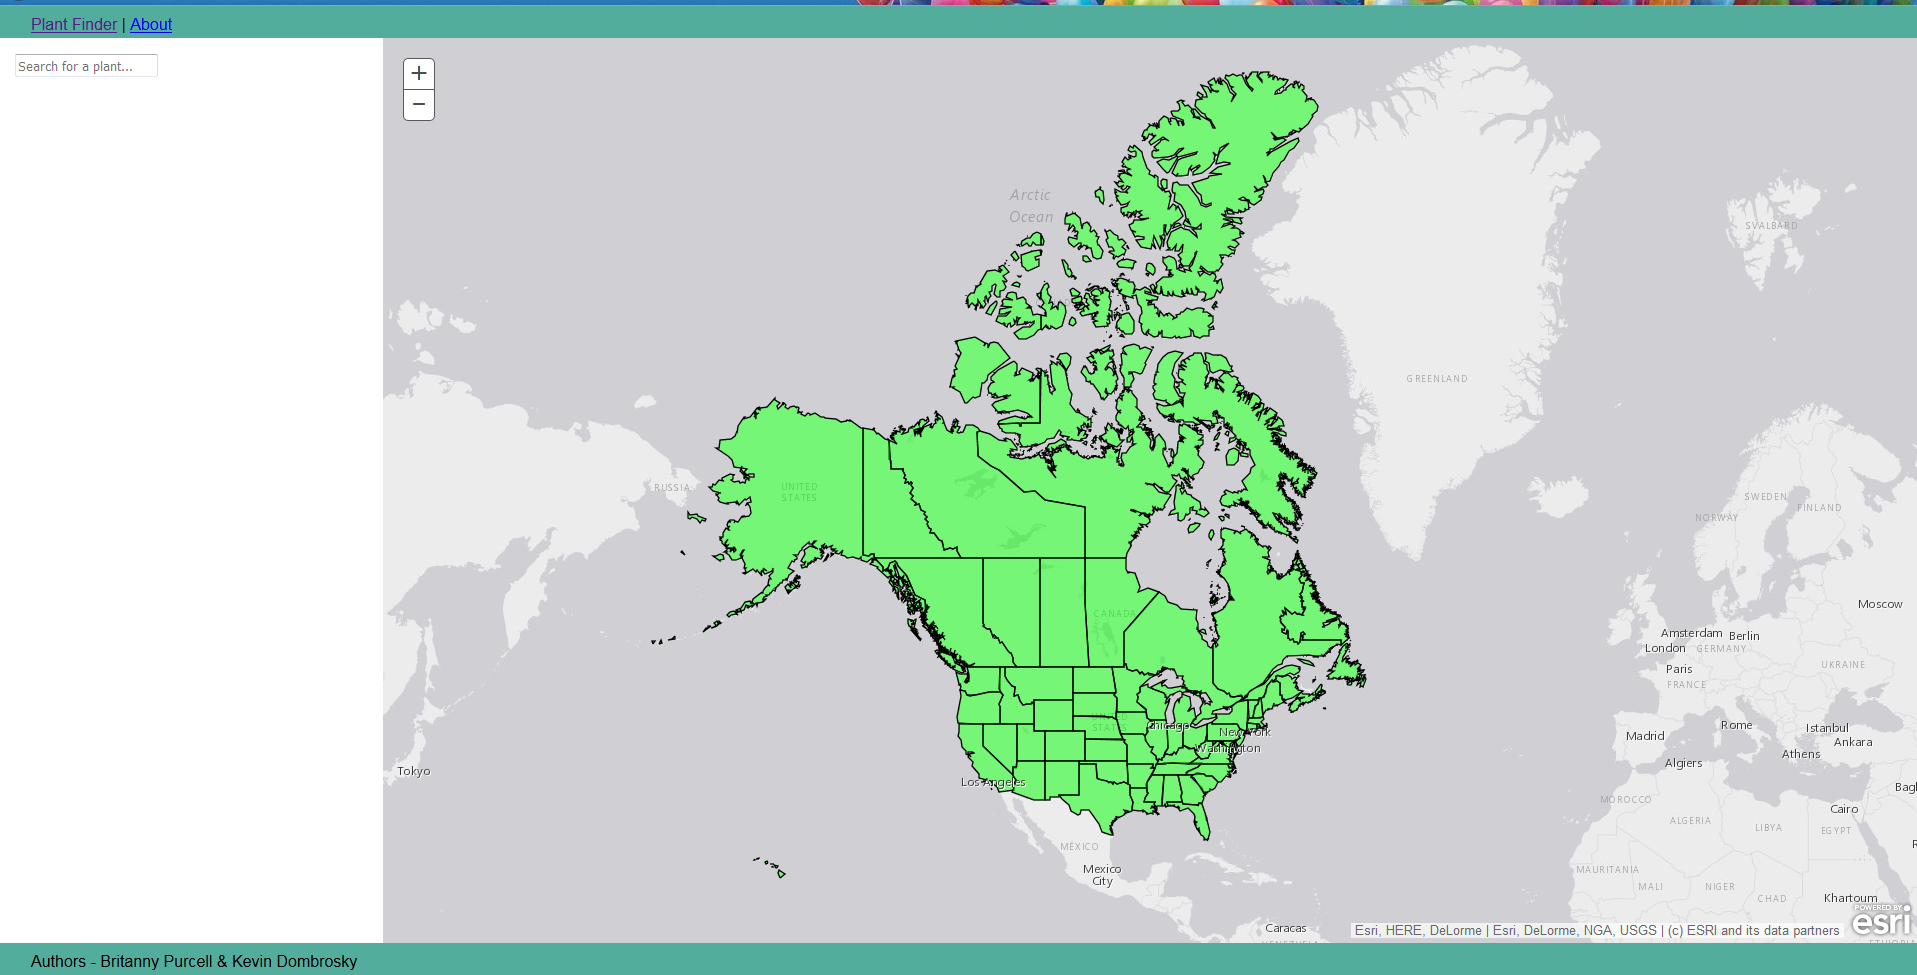
\includegraphics[scale=0.17]{Website_Screenshot.png}
	\caption{The blueprint for the website.}
\end{figure}


This application is a web page that was written in Jade Markup Language with CSS. This is the language that is most familiar to the group, after one of the members worked with the language all summer on an independent project. The basic blueprint for the web page can be seen (Figure 2), and in Figure 3 is the final result of the webpage.

\begin{figure}[htb]
	\centering
	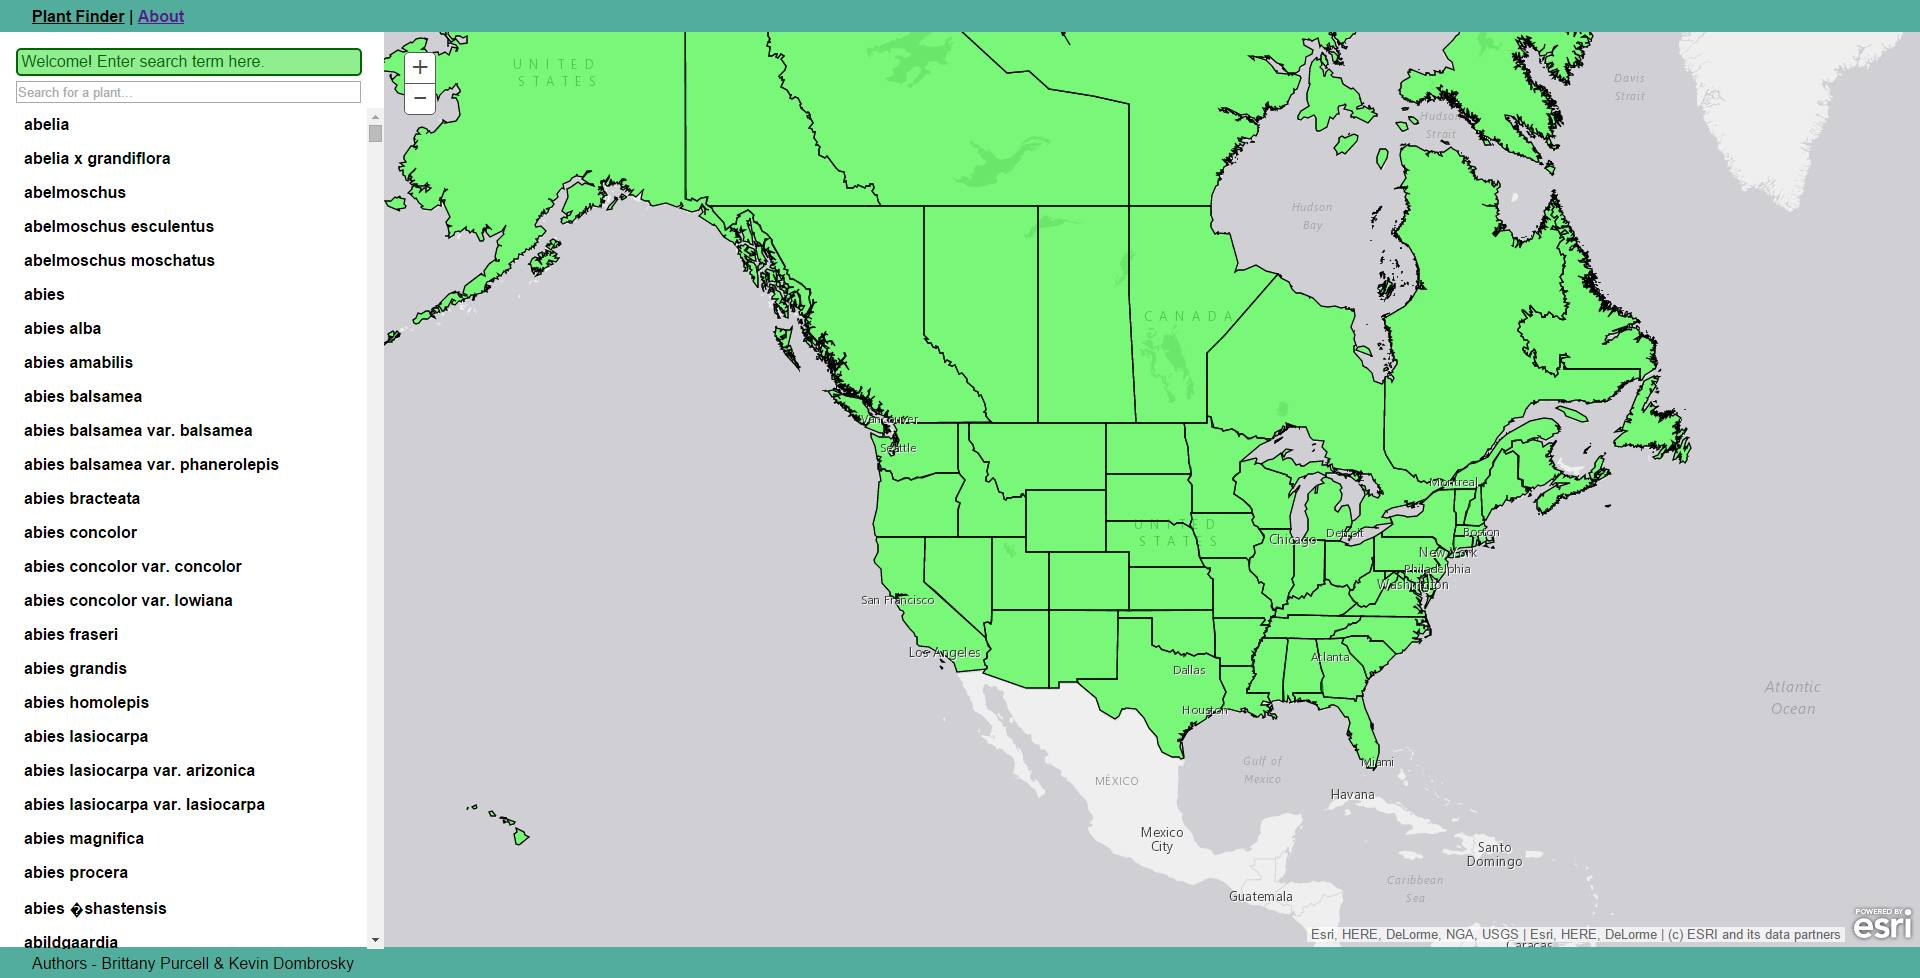
\includegraphics[scale=0.12]{finalScreenshot.jpg}
	\caption{The final website.}
\end{figure}


\subsection{Communication}
In order to allow communication between the webpage and the database, the data needed to be uploaded to a server. The members used a Node.js server, and using the Jade Markup Language with CSS the group could make calls to the server requesting data. The data is then transmitted to the webpage, and the results are displayed on the webpage. 

In order to make the communication work the group used a MySQL package that would allow for communication. In order to secure and protect this information a protect SQL injection with the escape command was used.

There are a few areas where the group had to create slight workarounds in order to get the information to display nicely. There was a schema name change part of the way through the project in order to make the information easier to access. Also, there was a slight problem with Newfoundland and Labrador. These locations were seperate in the database, but are the same place on the map. In order to compensate for this and display the information correctly, at runtime if the database requests information for the location, it will pull the information from both Newfoundland and Labrador and combine the results. These results will then be displayed at one place. This is the same if a plants location is either Labrador or Newfoundland. Either way, if one or both, the location would be marked as an available place for the plant. 

\subsection{Resources}
There were many resources that were used in order to develop and complete the project. These include certain files, softwares, and online databases. 
The database was set up using a MySQL database, and the visualization is coded using Jade and CSS. THe database and webpage communicate using a Node.js Server. The communication is protected and available because of MySQL packages and protected SQL injections.

The code and files are all being stored using GitHub which is accessible by all of the members of the group. GitHub is a repository to store, download, and change the existing code. The code itself was written using many different platforms. Some members used Notepad++, while others are using Visual Studio Code. Any changes to files or code needed to be pushed to the repository.

LaTeX is being used to write the ACM style templates, which is the document you are currently reading, and Visual Studio Code/Notepad++ is used for the README(which will walk users through how to run the program and access the website).

The README will be provided to establish step-by-step instructions on downloading and installing necessary software, and (once the software is installed), how to run the project and access the website. 


\section{Conclusions}
The group has successfully created a working webpage visualization which will allow analysis on a large dataset of plant information. They designed and implemented a worker database set up on a usable and accessible server. Information has been moved, copied, and rearranged to create the database, and the visualization has been adapted to work with the data.

Below is a list of all of the different elements that needed to be accomplished in order to create the final project. There is also a simple list of the resources that were used by the group to make the project possible. Many of these recourses were mentioned previously in the paper, but this is a full list of them. Lastly, is all of the necessary files and folders that should be available in the zip folder. These are important for the explanation of the project, the README describing the process needed to set everything up, and this document.

\begin{description}
	\item[Work Done:] \hfill
	\begin{itemize}
		\item Developed ER Diagram
		\item Created Website Wire Frame
		\item Setup Website
		\item Conceptualized Application Utilization
		\item Write Python Script for Database Input
		\item Set Up Database
		\item Establish Communication Between Website and Database
		\item Display Information on Website
		\item Change Display based on User Input
	\end{itemize}
	
	\item[Resources] \hfill
	\begin{itemize}
		\item GitHub
		\item LaTeX
		\item Node.js
		\item Notepad++
		\item Visual Studio Code
	\end{itemize}
	
	\item[Files] \hfill
	\begin{itemize}
		\item README
		\item Group6-Phase2
		\item CSCI620-master (Folder)
	\end{itemize}
\end{description}


\end{document}  % This is where a 'short' article might terminate
